\chapter{Introduction}
\label{chap:intro}
Information extraction (IE) from the web pages is a popular task which often occurs on the stage of data collection for further building of statistical model or other data processing procedures. The goal of IE is the automatic extraction of structural data from unstructured or semi-structured one. In general case, IE algorithm should \textit{learn how} to extract the meaningful structural information from training labeled data and then be able to do the same on previously unseen data with reasonable quality. This formulation basically allows considering IE problem as a machine learning task.

IE is closely related to Information Retrieval (IR) task. The purpose of IR is for a particular query to select and rank a subset of documents from the corpus of textual documents. Selected documents are relevant and ranked which is very convenient but at this point, no relevant information is being extracted. That's exactly where IE is applied. In order to extract the facts or meaningful information one need to understand the semantic of the documents.\\

IE task considered to be more difficult than IR. However, IR and IE techniques are complementary and may be combined in different ways. IE often uses the IR as a filtering step, because usually, the corpus of texts where the IE is extracting the information from is very large.\\

\cite{IEstate}




\section{Motivation}
Besides the obvious IE application in the search engine, there are also so-called vertical web services where IE is widely used too. Such websites allow to explore and work with the information on a specific topic. Such services usually do not produce the content by themselves, rather they automatically collect the data from various sources, processes this data in some way and present to the user in the appealing form. Such services also called \textit{aggregators}. A broad list of topics includes news, retail and other advertisements, reviews, flight tickets, videos and pictures, recipes, social networks and many other. The list is very extensive, virtually for any topic discussed and presented on the Internet there are aggregators exist which try to grasp all other sources into one. \\

Aggregators are usually very popular because they provide the user with the big database, rich functionality, flexibility and instant updates, what helps a user to save time. Due to popularity of aggregator the 'original' content maker is becoming popular too and therefore the content maker has resources to produce new interesting content. The other side of this practice is traffic reduction on the original content maker websites. It happens for example if the aggregator is unfair and doesn't show the source of the information. \\

The relationship between aggregators and original source makers today reminds the problem of chicken and egg. That's why search engines are very accurate with automatic extraction at the moment of showing the result for the search query. If Google shows you the correct answer right when you type the question, the website with this particular answer where Google took the information from will lose the user. Since this site loses the user, it also loses monetizing and resources to produce the 'correct answers' in future, this Google will lose the sources of correct answers. That's the reason why IE among Internet industry players is a controversial topic.\\

In research area, IE of web pages is usually used in the tasks related to natural language processing and text mining. The reason for this is that the web page content is basically the semi-structured text mixed with the HTML markdown. Many research project centered around the analysis of various news sources as news articles, tweets, social networks, etc. Here is an incomplete list of possible tasks: sentiment analysis of news, topic recognition, summarization. Some projects aim to build the system which determines the answer on human-language question based on huge amount of processed text (IBM Watson, Wolfram Language).\\      

The extraction of data from the web page is usually linked with the Document Object Model (DOM) processing and implies the understanding of the web page structure from the 'browser' point of view. \\

In this way, IE is becoming a quite interesting, actual and challenging task. It includes both the technical background for the data retrieving and manipulation as well as theoretical background for the reasonable model building. This thesis includes all necessary parts of this task.

\section{Problem definition}
In the thesis, we aim to create the system which automatically extracts the \textit{event components} of the social events from the web page. The social events might include musical concerts, meetings, performances, festivals, cinema and other social activities. Such events may be published on the different websites, usually on a website of the event organizer.\\

To classify the entity on a web page as an event let's state that it must have the following \textit{event components}:
\begin{enumerate}
    \item The title
    \item The description
    \item The date and time
    \item Certain location where event is taking place
\end{enumerate}

In this thesis, we won't solve the problem of identifying if the event announcement is actually placed on the web page since it is the task from IR field. We assume that the page already has an event and we want to find and extract the structured information about it (i.e. extract four items above).\\

We consider \textit{the webpage} as the already rendered page where JavaScript is executed. Such page has several important components: DOM tree, corresponding CSS, HTML code, resources (e.g. images) and rendered picture which the browser displays us. For one webpage we will collect all web elements from a DOM and four of them would be components we need to extract. We will collect more than two hundreds features for every web element and try to build the model which distinguishes an event components from all other elements. In such way for every event component we will build the binary classifier. That means in our problem we will build four one-vs-all classifiers where each of them will refers and detects corresponding event component. 

\begin{figure}[h]
\begin{center}
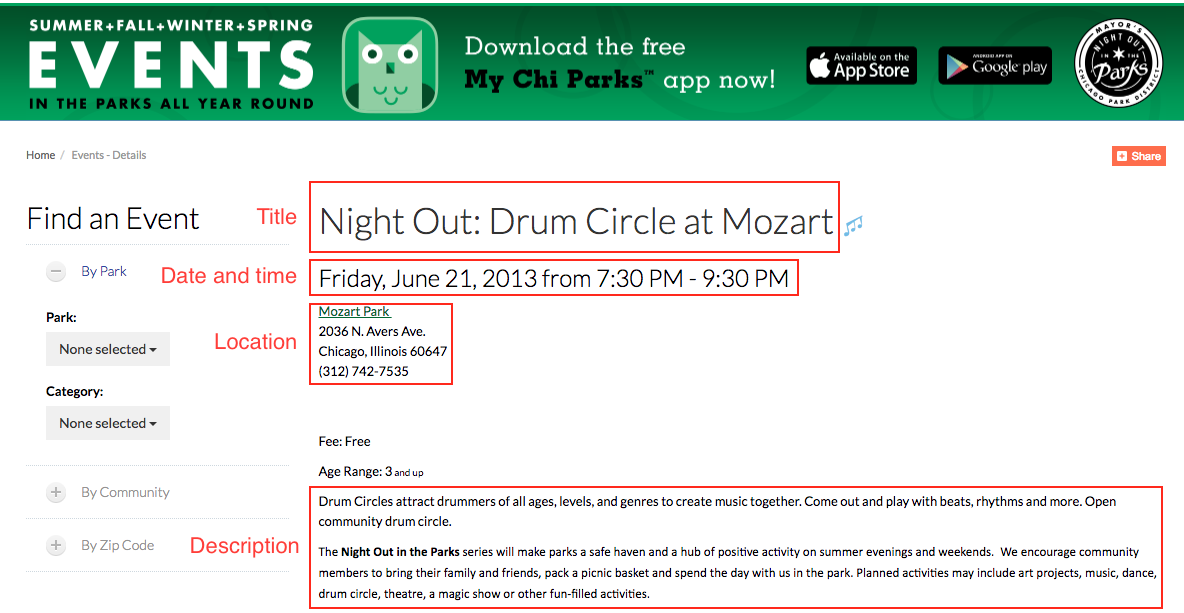
\includegraphics[width=1.0\textwidth]{figures01/event_example}
\caption{An example of the social event on a webpage. Four main event components are circled in red.}
\label{fig:architecture}
\end{center}
\end{figure}



\section{Objective and Contributions}

\section{Thesis Outline / TODO}
The thesis consists of 8 chapters, \nameref{append} and \nameref{chap:cd}. 
The current Chapter \ref{chap:intro}: \nameref{chap:intro} describes briefly the idea of the thesis and motivation for the task of automatic information extraction. Below you see the summary of all other chapters:
 
\subsection* {Chapter \ref{chap:background}: \nameref{chap:background}}
This chapter will cover necessary theoretical background. We will give definitions of major concepts which we are going to work with. First of all we will consider the structure of a webpage which is essential for this work, specially the notion of the Documnet Object Model (DOM) and it's relation with JavaScript and HTML. Then we will provide an overview of state of the art Information Extraction techniques and the reference to related work. The crucial part of the chapter is the notion of Microdata semantic markup. In fact the Microdata markup provides the basis of the thesis, namely, collecting the training dataset.  

\subsection* {Chapter \ref{chap:design}: \nameref{chap:design}}
\subsection* {Chapter \ref{chap:datacollect}: \nameref{chap:datacollect}}
\subsection* {Chapter \ref{chap:dataexplore}: \nameref{chap:dataexplore}}
\subsection* {Chapter \ref{chap:model}: \nameref{chap:model}}
\subsection* {Chapter \ref{chap:eval}: \nameref{chap:eval}}
\subsection* {Chapter \ref{chap:conclusion}: \nameref{chap:conclusion}}